\documentclass[letterpaper]{article}
\usepackage[utf8]{inputenc}
\usepackage[T1]{fontenc}
\usepackage[activeacute,english]{babel}
\usepackage[vmargin=4cm,tmargin=3cm,hmargin=2cm,letterpaper]{geometry}%
\usepackage{helvet}
\usepackage{amsmath,amsfonts,amssymb}
\usepackage{graphicx}
\usepackage{color}
\usepackage{xcolor}
\usepackage{verbatim}
\usepackage{tabls}
\usepackage{lastpage}
\usepackage{fancyhdr}
\usepackage{url}
\usepackage{listings}
\usepackage{tikz}
\usepackage{pgf}
\usepackage{pgffor}
\usepgfmodule{plot}
\usepackage{wrapfig}
\usepackage{ifpdf}
\usepackage{amssymb}
\usepackage{pifont}
\usepackage{epstopdf}
\usepackage{graphicx} % Allows including images
\usepackage{booktabs} % Allows the use of \toprule, \midrule and \bottomrule in tables
\usepackage{tikz}
\usetikzlibrary{arrows,decorations,snakes,backgrounds,fit,calc,through,scopes,positioning,automata,chains,er,fadings,calendar,matrix,mindmap,folding,patterns,petri,plothandlers,plotmarks,shadows,shapes,shapes.arrows,topaths,trees}

\lstset{% general command to set parameter(s)
%   basicstyle=\small,
  % print whole listing small
%   keywordstyle=\color{black}\bfseries\underbar,
  % underlined bold black keywords
%   identifierstyle=,
  % nothing happens
%   commentstyle=\color{white}, % white comments
%   stringstyle=\ttfamily,
  % typewriter type for strings
  showstringspaces=false}
  % no special string spaces

\pagestyle{fancy}
\color{black}
\fancyhead{}
\renewcommand{\headrule}{\hrule\vspace*{0.5mm}\rule{\linewidth}{0.8mm}}
\renewcommand{\familydefault}{\sfdefault}

\graphicspath{{./images/}}
\lhead{
\includegraphics[width=2cm]{logoucr.png}}
\rhead{
\includegraphics[width=3cm]{eie-text-gray-6x3cm.png}}
\chead{UNIVERSIDAD DE COSTA RICA\\FACULTAD DE INGENIERÍA\\ESCUELA DE INGENIERÍA ELÉCTRICA\\\textbf{ESTRUCTURAS ABSTRACTAS DE DATOS Y\\ ALGORITMOS PARA INGENIERÍA}\\IE-0217\\I CICLO 2014\\PROPUESTA DE PROYECTO ESTRUCTURAS DE DATOS}

\lfoot{}%
\cfoot{}%
%\cfoot{\thepage\ de \pageref{LastPage}}%
\rfoot{}%

%%%%%%%%%%%%%%%%%%%%%%%%%%%%%%%%%%%%%%%%%%%%%%%%%%%%%%%%%%%%%%%%%%%%%%%%%%%%%%%%%%%%%%%%%%%%%%%%%%%%%%%%%%%%%%%
\newcommand{\uic}{blue} %user-input color
%%%%%%%%%%%%%%%%%%%%%%%%%%%%%%%%%%%%%%%%%%%%%%%%%%%%%%%%%%%%%%%%%%%%%%%%%%%%%%%%%%%%%%%%%%%%%%%%%%%%%%%%%%%%%%%%%%
\newcommand{\uim}{\_\_} %user-input marker
%%%%%%%%%%%%%%%%%%%%%%%%%%%%%%%%%%%%%%%%%%%%%%%%%%%%%%%%%%%%%%%%%%%%%%%%%%%%%%%%%%%%%%%%%%%%%%%%%%%%%%%%%%%%%%%%%%
\newcommand{\userinput}[1]{\textcolor{\uic}{\uim#1\uim}}


%%%%%%%%%%%%%%%%%%%%%%%%%%%%%%%%%%%%%%%%%%%%%%%%%%%%%%%%%%%%%%%%%%%%%%%%%%%%%%%%%%%%%%%%%%%%%%%%%%%%%%%%%%%%%%%%%%
\begin{document}\vspace*{2cm}
%%%%%%%%%%%%%%%%%%%%%%%%%%%%%%%%%%%%%%%%%%%%%%%%%%%%%%%%%%%%%%%%%%%%%%%%%%%%%%%%%%%%%%%%%%%%%%%%%%%%%%%%%%%%%%%%%%

%%%%%%%%%%%%%%%%%%%%%%%%%%%%%%%%%%%%%%%%%%%%%%%%%%%%%%%%%%%%%%%%%%%%%%%%%%%%%%%%%%%%%%%%%%%%%%%%%%%%%%%%%%%%%%%%%%
\begin{center}
\Huge
\textbf{Kinect Data Library}
\vspace*{1cm}
\end{center}

\noindent
\small\baselineskip=14pt
\textbf{Estudiantes:} \\
\text{David Pérez Bolaños - B04769}\\
\text{Andrey Pérez Salazar - B25084}\\
\text{Andrés Sánchez López - B26214}\\


%\begin{figure}[ht]
%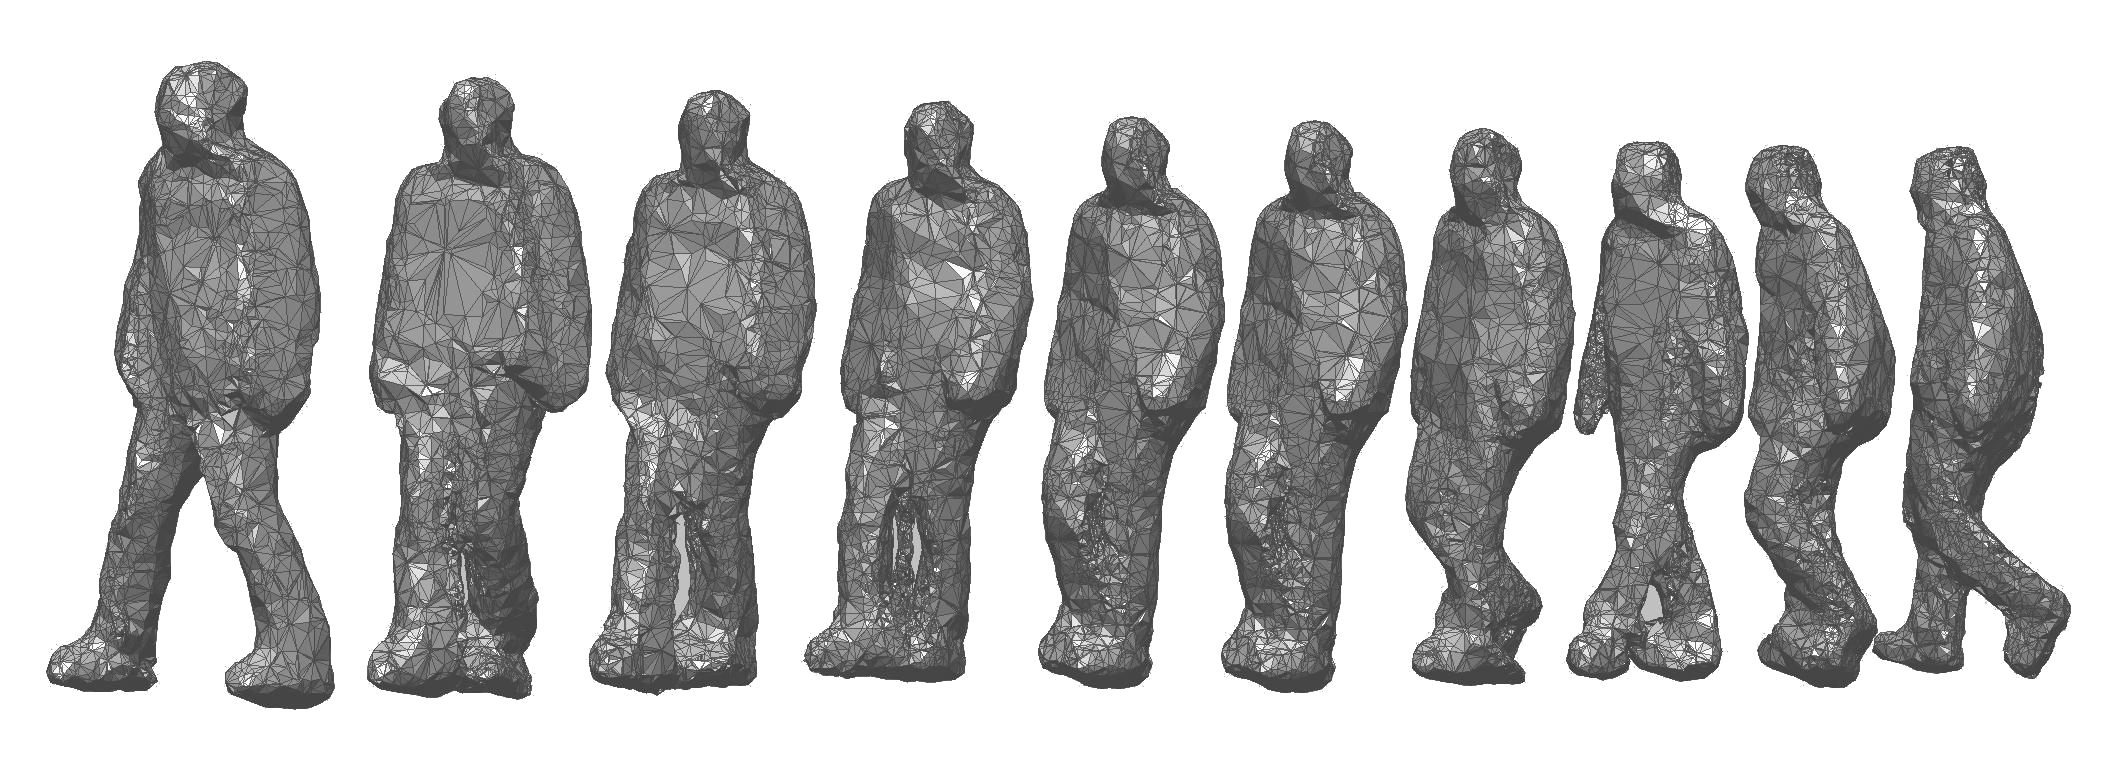
\includegraphics[width=1\linewidth]{visual_hull_4.png}
%\end{figure}


%%%%%%%%%%%%%%%%%%%%%%%%%%%%%%%%%%%%%%%%%%%%%%%%%%%%%%%%%%%%%%%%%%%%%%%%%%%%%%%%%%%%%%%%%%%%%%%%%%%%%%%%%%%%%%%%%%
\section{Introducción}
\hyphenation{fun-cio-na-li-dad}
Una estructura de datos es ... (No tengo idea)

%%%%%%%%%%%%%%%%%%%%%%%%%%%%%%%%%%%%%%%%%%%%%%%%%%%%%%%%%%%%%%%%%%%%%%%%%%%%%%%%%%%%%%%%%%%%%%%%%%%%%%%%%%%%%%%%%%
\section{Objetivos}

\subsection{Objetivo General}


El objetivo general consiste en .\\


\subsection{Objetivos Específicos}

Los objetivos específicos son:\\

\begin{enumerate}
\item Ampliar el conocimiento de. 
\item Desarrollar .
\item Obtener .
\end{enumerate}

%%%%%%%%%%%%%%%%%%%%%%%%%%%%%%%%%%%%%%%%%%%%%%%%%%%%%%%%%%%%%%%%%%%%%%%%%%%%%%%%%%%%%%%%%%%%%%%%%%%%%%%%%%%%%%%%%%
\section{Metodología}


Se realizará 

%%%%%%%%%%%%%%%%%%%%%%%%%%%%%%%%%%%%%%%%%%%%%%%%%%%%%%%%%%%%%%%%%%%%%%%%%%%%%%%%%%%%%%%%%%%%%%%%%%%%%%%%%%%%%%%%%%


\section{Cronograma}

\begin{center}
\begin{tabular}{l l   @{\hspace{1cm}}p{10cm}}
\cline{3-3}

\toprule
\textbf{Semana} & \textbf{Fechas} & \textbf{Actividad} \\
\midrule
1 & 28 de abril a 4 de mayo & Estudio  \\
2 & 5 de mayo a 14 de mayo & Desarrollo \\

3 & 15 de mayo a 17 de mayo & Prueba \\
4 & 19 de mayo a 19 de mayo & Realización  \\
\bottomrule
\end{tabular}
\end{center}

\begin{figure}[ht]
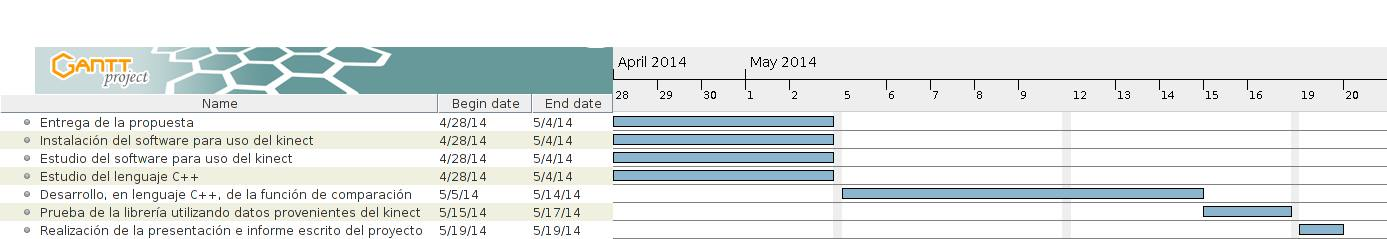
\includegraphics[width=1\linewidth]{10288526_791857134159417_2036565498_o.jpg}
\end{figure}

\section{Referencias}

\begin{enumerate}

\item Ri
\item E
\item O

\end{enumerate}

	
\end{document}

